\documentclass[border=5pt]{standalone}
\usepackage{tikz}
\usetikzlibrary{patterns,backgrounds}

\begin{document}
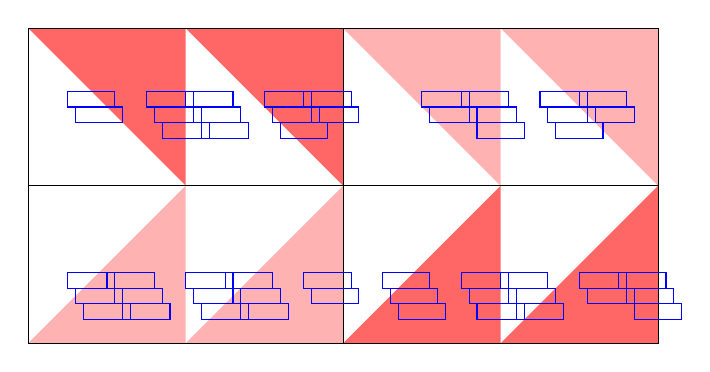
\begin{tikzpicture}

% 定义小矩形堆叠结构
\newcommand{\blockstructure}[3]{% x, y, 类型
  \begin{scope}[shift={(#1,#2)}]
    \ifcase#3% 类型0 - 3层
      \draw[blue] (0,0) rectangle (0.6,0.2);
      \draw[blue] (0.1,-0.2) rectangle (0.7,0);
      \draw[blue] (0.2,-0.4) rectangle (0.8,-0.2);
    \or% 类型1 - 4层
      \draw[blue] (0,0) rectangle (0.6,0.2);
      \draw[blue] (0.1,-0.2) rectangle (0.7,0);
      \draw[blue] (0.2,-0.4) rectangle (0.8,-0.2);
      \draw[blue] (0.3,-0.6) rectangle (0.9,-0.4);
    \or% 类型2 - 2层
      \draw[blue] (0,0) rectangle (0.6,0.2);
      \draw[blue] (0.1,-0.2) rectangle (0.7,0);
    \fi
  \end{scope}
}

% 绘制背景
\begin{scope}[on background layer]
  % 左上角深色区域
  \fill[red!60] (0,4) -- (2,4) -- (2,2) -- (0,4);
  \fill[red!60] (2,4) -- (4,4) -- (4,2) -- (2,4);
  % 右上角浅色区域
  \fill[red!30] (4,4) -- (6,4) -- (6,2) -- (4,4);
  \fill[red!30] (6,4) -- (8,4) -- (8,2) -- (6,4);
  % 左下角浅色区域
  \fill[red!30] (0,0) -- (2,0) -- (2,2) -- (0,0);
  \fill[red!30] (2,0) -- (4,0) -- (4,2) -- (2,0);
  % 右下角深色区域
  \fill[red!60] (4,0) -- (6,0) -- (6,2) -- (4,0);
  \fill[red!60] (6,0) -- (8,0) -- (8,2) -- (6,0);
  
  % 填充边缘区域
  \fill[red!30] (0,4) rectangle (0,0);
  \fill[red!30] (8,4) rectangle (8,0);
\end{scope}

% 绘制矩阵网格
\draw (0,0) rectangle (8,4);
\draw (4,0) -- (4,4);
\draw (0,2) -- (8,2);

% 绘制第一象限的块结构
\blockstructure{1.5}{3}{0}
\blockstructure{3}{3}{0}
\blockstructure{5}{3}{2}
\blockstructure{6.5}{3}{0}

% 绘制第二象限的块结构
\blockstructure{0.5}{3}{2}
\blockstructure{2}{3}{0}
\blockstructure{3.5}{3}{2}
\blockstructure{5.5}{3}{0}
\blockstructure{7}{3}{2}

% 绘制第三象限的块结构
\blockstructure{1}{0.7}{0}
\blockstructure{2.5}{0.7}{0}
\blockstructure{4.5}{0.7}{0}
\blockstructure{6}{0.7}{0}
\blockstructure{7.5}{0.7}{0}

% 绘制第四象限的块结构
\blockstructure{0.5}{0.7}{0}
\blockstructure{2}{0.7}{0}
\blockstructure{3.5}{0.7}{2}
\blockstructure{5.5}{0.7}{0}
\blockstructure{7}{0.7}{2}

\end{tikzpicture}
\end{document}